\SourceLeaf{204}\begin{center}Beispiel an der Theorie des Nivellirens einer Ebene.\end{center}


\begin{center}
\begin{minipage}[t]{.52\linewidth}\centering\textls{[H(orizont) und T(isch)]}\\[8pt]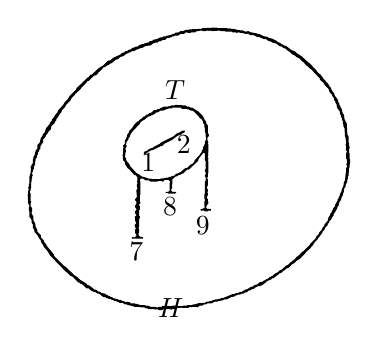
\begin{tikzpicture}[x=0.00726073cm,y=-0.00726073cm]
\fill[even odd rule] (491,391) -- (484,388) -- (475,381) -- (471,380) -- (469,378) -- (467,378) -- (465,376) -- (460,374) -- (458,372) -- (450,368) -- (445,367) -- (442,365) -- (436,364) -- (428,360) -- (425,360) -- (424,359) -- (413,357) -- (409,355) -- (404,356) -- (400,354) -- (389,353) -- (388,352) -- (385,352) -- (384,351) -- (378,351) -- (377,350) -- (373,351) -- (372,350) -- (355,350) -- (354,349) -- (344,349) -- (343,350) -- (338,349) -- (337,350) -- (328,350) -- (327,351) -- (305,352) -- (304,353) -- (299,353) -- (295,355) -- (290,355) -- (288,357) -- (281,358) -- (279,360) -- (277,360) -- (273,362) -- (270,362) -- (269,363) -- (266,363) -- (265,364) -- (261,364) -- (258,366) -- (255,366) -- (249,369) -- (243,370) -- (241,372) -- (236,373) -- (234,375) -- (228,376) -- (227,377) -- (219,379) -- (215,382) -- (212,382) -- (209,384) -- (207,384) -- (203,387) -- (199,388) -- (197,390) -- (194,390) -- (192,392) -- (187,394) -- (185,396) -- (172,402) -- (168,406) -- (166,406) -- (162,408) -- (155,415) -- (147,420) -- (135,431) -- (133,431) -- (129,436) -- (128,436) -- (121,443) -- (120,443) -- (119,445) -- (108,455) -- (108,457) -- (96,469) -- (93,474) -- (88,479) -- (85,484) -- (76,494) -- (75,497) -- (70,503) -- (70,504) -- (66,509) -- (65,512) -- (62,515) -- (62,517) -- (55,525) -- (53,532) -- (49,536) -- (49,538) -- (46,542) -- (44,550) -- (40,554) -- (40,560) -- (37,564) -- (35,572) -- (33,575) -- (33,578) -- (32,579) -- (32,586) -- (30,588) -- (30,590) -- (28,592) -- (29,598) -- (28,599) -- (28,604) -- (27,605) -- (27,608) -- (26,609) -- (26,622) -- (25,623) -- (25,627) -- (24,628) -- (25,633) -- (24,634) -- (24,640) -- (23,641) -- (24,656) -- (26,660) -- (26,662) -- (25,663) -- (25,669) -- (26,670) -- (26,680) -- (28,682) -- (30,686) -- (30,690) -- (32,693) -- (32,699) -- (34,701) -- (35,706) -- (41,713) -- (42,716) -- (46,721) -- (47,725) -- (50,729) -- (51,732) -- (58,740) -- (62,747) -- (91,777) -- (92,777) -- (98,783) -- (101,784) -- (112,795) -- (114,795) -- (116,797) -- (119,798) -- (125,804) -- (127,805) -- (130,805) -- (133,808) -- (139,811) -- (141,811) -- (145,814) -- (148,814) -- (154,819) -- (156,820) -- (159,820) -- (161,822) -- (163,822) -- (164,823) -- (168,823) -- (170,825) -- (172,825) -- (175,827) -- (177,827) -- (184,830) -- (189,830) -- (193,833) -- (197,833) -- (198,834) -- (204,835) -- (205,836) -- (208,836) -- (209,837) -- (219,837) -- (220,838) -- (227,838) -- (230,840) -- (233,840) -- (234,841) -- (245,841) -- (246,842) -- (250,841) -- (252,843) -- (257,843) -- (261,841) -- (272,841) -- (273,842) -- (275,842) -- (276,841) -- (283,841) -- (285,839) -- (290,839) -- (291,838) -- (293,839) -- (304,839) -- (307,837) -- (309,838) -- (311,837) -- (318,837) -- (320,838) -- (324,835) -- (328,835) -- (331,833) -- (335,833) -- (337,831) -- (345,831) -- (350,828) -- (355,828) -- (356,827) -- (363,826) -- (367,824) -- (371,824) -- (379,820) -- (385,819) -- (387,817) -- (389,817) -- (390,816) -- (394,816) -- (397,814) -- (401,814) -- (403,812) -- (406,812) -- (409,809) -- (413,808) -- (415,806) -- (418,806) -- (420,804) -- (426,801) -- (429,801) -- (435,798) -- (442,792) -- (449,789) -- (451,787) -- (453,787) -- (459,782) -- (460,782) -- (464,778) -- (466,778) -- (470,774) -- (471,774) -- (476,770) -- (479,769) -- (486,762) -- (489,761) -- (494,756) -- (498,754) -- (509,743) -- (509,742) -- (518,734) -- (518,733) -- (522,729) -- (525,724) -- (531,718) -- (531,717) -- (538,708) -- (539,705) -- (542,702) -- (543,699) -- (547,695) -- (548,692) -- (550,690) -- (550,688) -- (554,684) -- (555,681) -- (558,678) -- (558,675) -- (561,671) -- (562,668) -- (564,666) -- (564,664) -- (567,659) -- (568,654) -- (571,650) -- (572,645) -- (574,642) -- (574,640) -- (576,636) -- (576,632) -- (577,631) -- (577,629) -- (579,627) -- (579,624) -- (582,618) -- (582,614) -- (583,613) -- (583,609) -- (584,608) -- (585,594) -- (586,593) -- (586,588) -- (587,587) -- (587,580) -- (586,579) -- (586,569) -- (585,568) -- (585,561) -- (586,560) -- (586,557) -- (585,556) -- (585,551) -- (584,550) -- (584,539) -- (582,536) -- (581,517) -- (577,509) -- (576,501) -- (574,499) -- (572,491) -- (570,488) -- (570,486) -- (568,484) -- (568,482) -- (566,479) -- (566,477) -- (564,473) -- (560,468) -- (559,464) -- (555,459) -- (553,454) -- (551,452) -- (549,448) -- (540,438) -- (540,437) -- (536,433) -- (536,432) -- (529,426) -- (529,425) -- (515,410) -- (514,410) -- (502,399) -- (494,394) -- cycle
(473,385) -- (480,391) -- (481,391) -- (486,396) -- (489,397) -- (494,401) -- (497,402) -- (504,409) -- (505,409) -- (511,416) -- (512,416) -- (517,421) -- (518,421) -- (534,438) -- (534,440) -- (540,445) -- (543,450) -- (549,456) -- (551,462) -- (555,466) -- (556,469) -- (559,473) -- (559,476) -- (561,478) -- (561,480) -- (563,483) -- (564,489) -- (569,496) -- (569,500) -- (571,502) -- (571,505) -- (573,508) -- (573,511) -- (574,512) -- (574,517) -- (575,518) -- (575,521) -- (577,525) -- (578,540) -- (579,541) -- (579,545) -- (580,546) -- (580,552) -- (579,553) -- (579,555) -- (580,556) -- (580,560) -- (579,562) -- (581,565) -- (581,567) -- (580,568) -- (580,578) -- (581,579) -- (581,586) -- (580,588) -- (581,589) -- (581,593) -- (580,594) -- (580,602) -- (579,603) -- (578,616) -- (576,619) -- (575,626) -- (572,632) -- (572,635) -- (569,640) -- (569,643) -- (567,645) -- (567,647) -- (565,649) -- (565,651) -- (560,660) -- (560,662) -- (557,665) -- (557,667) -- (555,669) -- (555,671) -- (552,675) -- (552,677) -- (550,679) -- (548,683) -- (548,686) -- (542,693) -- (542,695) -- (539,698) -- (537,703) -- (533,707) -- (532,710) -- (528,714) -- (526,718) -- (517,727) -- (517,728) -- (505,740) -- (504,740) -- (495,749) -- (494,749) -- (489,755) -- (488,755) -- (484,759) -- (483,759) -- (478,764) -- (475,765) -- (466,773) -- (464,773) -- (460,777) -- (457,778) -- (451,783) -- (446,785) -- (443,788) -- (440,789) -- (438,791) -- (436,791) -- (434,793) -- (429,794) -- (424,798) -- (420,799) -- (416,802) -- (414,802) -- (410,804) -- (408,806) -- (404,807) -- (397,811) -- (394,811) -- (391,813) -- (388,813) -- (384,815) -- (381,815) -- (364,822) -- (361,822) -- (360,823) -- (357,823) -- (356,824) -- (351,824) -- (350,825) -- (348,825) -- (344,827) -- (341,827) -- (340,828) -- (337,828) -- (333,830) -- (320,831) -- (319,832) -- (317,832) -- (316,833) -- (312,833) -- (311,834) -- (302,834) -- (301,835) -- (295,835) -- (294,836) -- (286,836) -- (285,835) -- (276,835) -- (275,836) -- (258,836) -- (257,837) -- (252,837) -- (251,838) -- (248,838) -- (247,837) -- (237,837) -- (236,836) -- (234,836) -- (233,835) -- (229,835) -- (228,834) -- (219,834) -- (218,833) -- (215,833) -- (214,832) -- (211,832) -- (210,831) -- (203,831) -- (201,829) -- (198,829) -- (197,828) -- (194,829) -- (191,827) -- (189,827) -- (185,825) -- (182,825) -- (181,824) -- (173,822) -- (170,820) -- (168,820) -- (166,818) -- (164,818) -- (162,816) -- (160,816) -- (158,814) -- (152,813) -- (150,811) -- (146,810) -- (142,807) -- (140,807) -- (131,800) -- (128,799) -- (125,796) -- (115,790) -- (107,783) -- (106,783) -- (88,766) -- (87,766) -- (69,748) -- (69,746) -- (56,730) -- (56,729) -- (52,724) -- (51,721) -- (47,717) -- (46,715) -- (46,712) -- (40,706) -- (40,703) -- (37,697) -- (36,691) -- (33,686) -- (33,680) -- (30,674) -- (30,671) -- (31,670) -- (31,665) -- (28,661) -- (28,656) -- (29,655) -- (29,653) -- (28,652) -- (28,639) -- (27,638) -- (27,635) -- (28,634) -- (28,631) -- (29,630) -- (29,619) -- (30,618) -- (30,613) -- (31,612) -- (31,608) -- (32,607) -- (31,605) -- (31,602) -- (32,601) -- (32,599) -- (34,595) -- (34,592) -- (36,588) -- (36,582) -- (37,581) -- (37,578) -- (39,576) -- (39,573) -- (41,570) -- (41,567) -- (43,565) -- (43,563) -- (45,561) -- (45,557) -- (50,549) -- (50,545) -- (51,543) -- (54,540) -- (55,537) -- (57,535) -- (59,531) -- (63,527) -- (64,525) -- (64,522) -- (70,516) -- (71,513) -- (73,511) -- (73,509) -- (75,507) -- (79,500) -- (82,497) -- (83,493) -- (88,488) -- (91,483) -- (98,476) -- (100,472) -- (106,466) -- (106,465) -- (116,456) -- (116,455) -- (126,445) -- (126,444) -- (128,442) -- (130,442) -- (139,433) -- (143,432) -- (146,429) -- (146,428) -- (154,421) -- (154,420) -- (156,418) -- (158,418) -- (162,415) -- (165,414) -- (167,412) -- (170,411) -- (177,405) -- (181,404) -- (185,400) -- (190,399) -- (195,395) -- (201,392) -- (203,392) -- (205,390) -- (209,390) -- (214,387) -- (216,387) -- (219,385) -- (224,384) -- (229,381) -- (238,380) -- (243,376) -- (245,376) -- (246,375) -- (250,375) -- (252,373) -- (255,373) -- (258,371) -- (264,370) -- (267,367) -- (271,367) -- (272,366) -- (274,366) -- (276,364) -- (279,364) -- (280,363) -- (286,363) -- (290,360) -- (296,360) -- (300,357) -- (302,357) -- (303,358) -- (308,358) -- (309,357) -- (316,357) -- (319,355) -- (323,355) -- (324,354) -- (328,354) -- (329,355) -- (335,355) -- (336,354) -- (339,354) -- (340,355) -- (342,354) -- (344,354) -- (345,355) -- (359,354) -- (360,355) -- (368,355) -- (369,356) -- (380,356) -- (381,357) -- (387,357) -- (388,358) -- (393,357) -- (394,358) -- (398,358) -- (399,359) -- (402,359) -- (403,360) -- (406,360) -- (408,359) -- (412,362) -- (418,362) -- (424,365) -- (427,365) -- (436,369) -- (440,369) -- (442,371) -- (446,373) -- (448,373) -- (451,375) -- (458,377) -- (463,381) -- (467,382) -- (471,385) -- cycle
(311,489) -- (308,489) -- (305,487) -- (302,487) -- (299,485) -- (281,484) -- (280,485) -- (274,485) -- (273,486) -- (270,486) -- (269,487) -- (260,487) -- (258,489) -- (256,489) -- (254,491) -- (251,491) -- (248,493) -- (244,493) -- (240,497) -- (235,499) -- (233,501) -- (231,501) -- (228,504) -- (225,505) -- (221,509) -- (220,509) -- (216,513) -- (215,513) -- (209,519) -- (206,524) -- (201,529) -- (199,534) -- (197,536) -- (197,539) -- (193,547) -- (193,552) -- (190,555) -- (190,557) -- (191,558) -- (190,560) -- (190,570) -- (189,571) -- (190,581) -- (193,584) -- (193,587) -- (198,595) -- (200,596) -- (210,607) -- (212,607) -- (215,611) -- (215,617) -- (214,618) -- (215,620) -- (215,622) -- (214,623) -- (214,628) -- (215,629) -- (215,631) -- (213,633) -- (214,645) -- (211,649) -- (211,651) -- (213,653) -- (213,657) -- (211,660) -- (211,663) -- (213,666) -- (213,668) -- (211,670) -- (211,674) -- (213,676) -- (213,677) -- (210,680) -- (211,682) -- (211,687) -- (212,688) -- (212,692) -- (210,694) -- (211,698) -- (212,699) -- (212,701) -- (211,702) -- (211,708) -- (213,711) -- (213,713) -- (210,716) -- (206,715) -- (205,716) -- (206,718) -- (224,718) -- (225,717) -- (224,715) -- (220,715) -- (217,712) -- (217,708) -- (218,707) -- (218,701) -- (217,700) -- (217,698) -- (218,697) -- (218,683) -- (219,682) -- (219,679) -- (218,678) -- (218,668) -- (219,667) -- (219,661) -- (218,660) -- (218,658) -- (220,656) -- (220,654) -- (219,653) -- (219,642) -- (220,641) -- (220,618) -- (219,617) -- (219,615) -- (221,613) -- (225,613) -- (229,616) -- (235,616) -- (238,618) -- (250,618) -- (251,617) -- (257,617) -- (258,618) -- (260,618) -- (263,615) -- (269,615) -- (272,618) -- (272,620) -- (271,621) -- (271,634) -- (269,636) -- (265,636) -- (264,637) -- (265,638) -- (268,638) -- (269,639) -- (281,639) -- (283,637) -- (282,636) -- (276,636) -- (274,634) -- (274,632) -- (276,628) -- (275,626) -- (275,624) -- (276,623) -- (276,614) -- (282,609) -- (284,609) -- (286,607) -- (288,607) -- (296,603) -- (302,597) -- (305,597) -- (321,582) -- (322,578) -- (330,568) -- (332,568) -- (333,569) -- (333,581) -- (334,582) -- (334,593) -- (335,594) -- (333,598) -- (333,600) -- (334,601) -- (334,606) -- (333,607) -- (333,609) -- (335,612) -- (334,614) -- (334,617) -- (333,618) -- (333,639) -- (332,640) -- (332,648) -- (333,649) -- (333,652) -- (332,653) -- (332,661) -- (333,663) -- (329,666) -- (326,666) -- (325,668) -- (326,669) -- (332,669) -- (333,670) -- (338,670) -- (339,669) -- (343,669) -- (344,668) -- (343,666) -- (337,666) -- (335,664) -- (336,660) -- (339,656) -- (339,654) -- (338,653) -- (338,649) -- (337,648) -- (337,643) -- (338,642) -- (338,638) -- (337,637) -- (338,635) -- (338,632) -- (337,631) -- (337,626) -- (338,625) -- (338,614) -- (337,613) -- (337,611) -- (338,610) -- (338,604) -- (339,603) -- (339,582) -- (338,581) -- (339,579) -- (339,577) -- (338,576) -- (338,573) -- (339,572) -- (339,570) -- (338,569) -- (339,567) -- (339,553) -- (338,551) -- (339,549) -- (338,548) -- (337,542) -- (340,538) -- (340,536) -- (338,533) -- (338,520) -- (335,516) -- (335,513) -- (333,511) -- (329,503) -- (322,496) -- cycle
(313,495) -- (323,505) -- (323,506) -- (328,510) -- (330,514) -- (330,516) -- (332,519) -- (332,523) -- (333,524) -- (333,532) -- (334,533) -- (334,539) -- (335,540) -- (335,545) -- (333,548) -- (333,552) -- (330,558) -- (330,561) -- (327,565) -- (327,567) -- (325,569) -- (325,570) -- (315,581) -- (314,584) -- (311,587) -- (307,589) -- (302,594) -- (298,595) -- (291,601) -- (285,604) -- (283,604) -- (279,608) -- (276,608) -- (273,610) -- (270,610) -- (269,611) -- (265,611) -- (264,612) -- (255,613) -- (254,614) -- (240,614) -- (239,613) -- (234,613) -- (233,612) -- (222,609) -- (217,605) -- (213,603) -- (202,591) -- (201,588) -- (196,582) -- (195,580) -- (195,577) -- (193,575) -- (193,573) -- (194,572) -- (194,567) -- (195,566) -- (194,560) -- (196,557) -- (196,555) -- (195,554) -- (196,548) -- (199,545) -- (199,543) -- (202,539) -- (202,537) -- (205,532) -- (219,517) -- (219,516) -- (223,512) -- (227,510) -- (233,505) -- (245,500) -- (248,497) -- (251,497) -- (255,494) -- (260,494) -- (261,493) -- (263,493) -- (266,491) -- (269,491) -- (270,490) -- (275,490) -- (276,489) -- (291,489) -- (293,491) -- (301,491) -- (302,492) -- (305,492) -- (308,494) -- (311,494) -- cycle
(298,530) -- (297,529) -- (294,529) -- (287,533) -- (285,533) -- (278,539) -- (256,550) -- (254,552) -- (244,557) -- (242,559) -- (238,560) -- (234,562) -- (232,564) -- (227,566) -- (226,567) -- (226,569) -- (227,570) -- (229,570) -- (234,566) -- (240,563) -- (242,563) -- (247,560) -- (249,560) -- (251,558) -- (253,558) -- (255,556) -- (258,556) -- (262,552) -- (276,545) -- (285,538) -- (291,536) -- (293,534) -- (297,532) -- cycle;
\node[inner sep=0pt] at (281,458) {$T$};
\node[inner sep=0pt] at (234,585) {$1$};
\node[inner sep=0pt] at (296,554) {$2$};
\node[inner sep=0pt] at (272,662) {$8$};
\node[inner sep=0pt] at (329,695) {$9$};
\node[inner sep=0pt] at (213,741) {$7$};
\node[inner sep=0pt] at (273,840) {$H$};
\end{tikzpicture}
\end{minipage}\hfill
\begin{minipage}[t]{.39\linewidth}\centering\textls{[Libelle]}\\[8pt]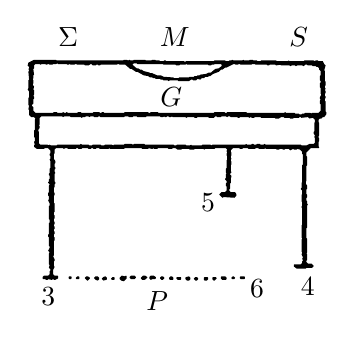
\begin{tikzpicture}[x=0.00898876cm,y=-0.00898876cm]
\fill[even odd rule] (276,705) -- (272,705) -- (271,706) -- (271,708) -- (273,710) -- (274,710) -- (277,707) -- cycle
(260,705) -- (259,706) -- (259,709) -- (260,710) -- (263,710) -- (265,708) -- (265,706) -- (264,705) -- cycle
(247,705) -- (245,707) -- (245,708) -- (247,710) -- (249,710) -- (251,708) -- (251,707) -- (249,705) -- cycle
(220,706) -- (220,707) -- (222,709) -- (226,709) -- (227,708) -- (227,706) -- (226,705) -- (221,705) -- cycle
(130,705) -- (128,707) -- (128,708) -- (129,709) -- (132,709) -- (133,708) -- (133,706) -- (132,705) -- cycle
(310,705) -- (310,707) -- (311,708) -- (316,708) -- (317,707) -- (317,705) -- (316,704) -- (311,704) -- cycle
(300,704) -- (298,706) -- (298,707) -- (299,708) -- (302,708) -- (303,706) -- (301,704) -- cycle
(283,705) -- (283,707) -- (285,709) -- (290,709) -- (291,708) -- (291,706) -- (289,704) -- (284,704) -- cycle
(234,705) -- (233,706) -- (233,708) -- (235,710) -- (238,710) -- (240,708) -- (240,706) -- (238,704) -- cycle
(212,704) -- (210,706) -- (210,708) -- (211,709) -- (215,709) -- (216,708) -- (216,706) -- (214,704) -- cycle
(199,704) -- (197,706) -- (197,707) -- (199,709) -- (201,709) -- (203,707) -- (203,706) -- (201,704) -- cycle
(120,704) -- (117,705) -- (115,707) -- (115,708) -- (117,710) -- (121,709) -- (122,708) -- (122,706) -- cycle
(106,704) -- (104,706) -- (104,707) -- (106,709) -- (109,710) -- (111,708) -- (111,706) -- (109,704) -- cycle
(93,704) -- (91,706) -- (91,707) -- (94,710) -- (95,710) -- (98,707) -- (98,706) -- (95,704) -- cycle
(80,704) -- (78,706) -- (78,707) -- (79,708) -- (82,708) -- (83,707) -- (83,705) -- (82,704) -- cycle
(69,704) -- (68,705) -- (68,707) -- (69,708) -- (71,708) -- (72,707) -- (72,705) -- (71,704) -- cycle
(182,705) -- (182,707) -- (184,709) -- (186,708) -- (190,708) -- (191,707) -- (191,705) -- (188,703) -- (184,703) -- cycle
(170,707) -- (172,709) -- (175,709) -- (177,708) -- (179,706) -- (179,705) -- (176,703) -- (173,703) -- (170,706) -- cycle
(154,705) -- (154,706) -- (156,708) -- (161,708) -- (163,706) -- (163,705) -- (161,703) -- (156,703) -- cycle
(149,703) -- (147,704) -- (143,703) -- (140,706) -- (140,708) -- (142,710) -- (146,711) -- (150,707) -- (150,704) -- cycle
(11,402) -- (10,406) -- (12,408) -- (12,410) -- (11,411) -- (12,413) -- (11,415) -- (12,426) -- (11,427) -- (11,438) -- (10,440) -- (12,443) -- (12,451) -- (11,452) -- (11,462) -- (12,463) -- (11,468) -- (12,469) -- (12,476) -- (15,479) -- (19,479) -- (21,481) -- (20,483) -- (20,497) -- (19,498) -- (19,507) -- (20,508) -- (20,513) -- (19,514) -- (20,518) -- (19,519) -- (19,521) -- (23,524) -- (33,524) -- (34,523) -- (39,523) -- (42,526) -- (42,530) -- (41,531) -- (41,533) -- (42,534) -- (42,538) -- (41,539) -- (42,541) -- (42,551) -- (41,552) -- (41,558) -- (40,559) -- (40,561) -- (41,562) -- (41,566) -- (40,567) -- (40,570) -- (39,571) -- (39,572) -- (41,574) -- (40,576) -- (40,585) -- (39,586) -- (39,590) -- (40,591) -- (40,595) -- (39,597) -- (41,601) -- (41,604) -- (40,605) -- (40,623) -- (41,624) -- (41,628) -- (40,629) -- (40,644) -- (39,645) -- (39,648) -- (40,649) -- (40,661) -- (41,662) -- (41,664) -- (39,668) -- (41,670) -- (40,672) -- (40,687) -- (41,688) -- (40,692) -- (42,694) -- (42,696) -- (41,697) -- (41,701) -- (39,703) -- (33,703) -- (31,705) -- (31,707) -- (32,708) -- (35,708) -- (36,709) -- (38,709) -- (39,708) -- (44,709) -- (46,708) -- (47,709) -- (49,709) -- (53,707) -- (53,704) -- (52,703) -- (48,703) -- (46,701) -- (46,695) -- (48,691) -- (47,689) -- (47,683) -- (48,682) -- (48,680) -- (46,676) -- (47,674) -- (47,654) -- (48,653) -- (48,649) -- (47,648) -- (47,645) -- (48,644) -- (48,641) -- (47,640) -- (47,638) -- (48,637) -- (48,634) -- (47,633) -- (47,631) -- (48,630) -- (48,627) -- (47,626) -- (47,623) -- (48,622) -- (48,618) -- (47,617) -- (47,614) -- (48,613) -- (48,601) -- (47,600) -- (47,590) -- (48,589) -- (48,586) -- (47,585) -- (47,579) -- (48,578) -- (48,574) -- (49,573) -- (49,571) -- (48,570) -- (48,559) -- (49,558) -- (48,556) -- (48,553) -- (49,552) -- (49,550) -- (48,549) -- (48,545) -- (49,544) -- (49,541) -- (47,538) -- (47,531) -- (48,530) -- (48,525) -- (50,523) -- (60,523) -- (61,524) -- (63,523) -- (66,523) -- (67,524) -- (78,524) -- (79,523) -- (81,523) -- (82,524) -- (86,524) -- (87,523) -- (95,523) -- (96,524) -- (99,524) -- (100,523) -- (102,523) -- (103,524) -- (106,524) -- (107,523) -- (111,523) -- (112,524) -- (124,524) -- (125,523) -- (127,524) -- (146,524) -- (147,523) -- (171,523) -- (172,524) -- (180,524) -- (181,523) -- (186,524) -- (188,523) -- (189,524) -- (193,524) -- (194,523) -- (208,523) -- (209,524) -- (214,524) -- (215,523) -- (219,523) -- (222,525) -- (227,525) -- (228,524) -- (238,524) -- (239,525) -- (245,525) -- (246,524) -- (258,524) -- (260,525) -- (261,524) -- (274,524) -- (275,523) -- (290,523) -- (292,525) -- (291,527) -- (292,529) -- (291,531) -- (291,533) -- (292,534) -- (292,539) -- (291,540) -- (291,551) -- (290,552) -- (290,557) -- (291,559) -- (290,560) -- (290,565) -- (289,566) -- (289,567) -- (291,569) -- (291,572) -- (290,573) -- (290,576) -- (291,577) -- (291,583) -- (289,585) -- (284,585) -- (281,588) -- (281,589) -- (285,593) -- (287,592) -- (302,593) -- (305,590) -- (305,588) -- (303,585) -- (297,585) -- (295,583) -- (295,581) -- (296,580) -- (296,573) -- (297,572) -- (297,565) -- (298,564) -- (298,562) -- (296,560) -- (296,559) -- (298,557) -- (297,555) -- (297,547) -- (298,546) -- (298,542) -- (297,541) -- (297,539) -- (298,538) -- (297,536) -- (297,534) -- (298,533) -- (298,529) -- (297,528) -- (297,526) -- (300,523) -- (309,523) -- (310,524) -- (313,524) -- (314,523) -- (321,523) -- (322,524) -- (331,524) -- (332,523) -- (336,523) -- (337,524) -- (344,524) -- (346,523) -- (347,524) -- (361,524) -- (362,525) -- (365,525) -- (366,524) -- (370,524) -- (371,525) -- (373,525) -- (374,524) -- (379,524) -- (381,526) -- (385,524) -- (387,525) -- (390,525) -- (391,524) -- (395,525) -- (398,528) -- (398,531) -- (399,532) -- (399,546) -- (398,547) -- (398,571) -- (397,572) -- (397,579) -- (396,580) -- (396,581) -- (398,583) -- (398,588) -- (397,589) -- (397,598) -- (398,599) -- (398,604) -- (397,605) -- (397,607) -- (398,608) -- (398,631) -- (397,632) -- (397,649) -- (398,651) -- (397,652) -- (397,669) -- (398,671) -- (397,673) -- (399,677) -- (398,679) -- (399,682) -- (398,683) -- (398,685) -- (396,687) -- (387,687) -- (386,688) -- (386,690) -- (390,693) -- (403,693) -- (404,692) -- (412,692) -- (414,690) -- (414,689) -- (411,686) -- (406,686) -- (404,684) -- (404,682) -- (405,681) -- (405,673) -- (404,672) -- (405,670) -- (405,651) -- (404,650) -- (404,636) -- (405,635) -- (405,604) -- (406,603) -- (405,601) -- (405,598) -- (404,597) -- (404,593) -- (405,592) -- (405,589) -- (404,588) -- (404,581) -- (405,580) -- (405,576) -- (403,573) -- (403,570) -- (404,569) -- (404,548) -- (405,547) -- (405,535) -- (404,534) -- (404,529) -- (410,523) -- (421,523) -- (422,522) -- (421,520) -- (421,514) -- (422,513) -- (422,509) -- (421,508) -- (421,506) -- (422,505) -- (422,487) -- (421,486) -- (421,483) -- (423,481) -- (425,481) -- (427,479) -- (429,479) -- (432,475) -- (432,472) -- (431,471) -- (431,457) -- (430,456) -- (430,453) -- (431,452) -- (431,450) -- (430,449) -- (430,446) -- (431,445) -- (431,442) -- (430,441) -- (431,439) -- (430,437) -- (430,435) -- (431,434) -- (431,429) -- (430,428) -- (430,414) -- (429,413) -- (431,406) -- (429,404) -- (427,400) -- (421,400) -- (420,399) -- (417,399) -- (416,400) -- (414,399) -- (401,399) -- (400,400) -- (380,400) -- (379,399) -- (377,400) -- (362,400) -- (361,399) -- (340,399) -- (339,400) -- (335,400) -- (334,399) -- (329,399) -- (328,398) -- (324,398) -- (323,399) -- (316,399) -- (315,398) -- (313,399) -- (301,399) -- (299,398) -- (298,399) -- (295,399) -- (294,400) -- (290,400) -- (289,399) -- (274,399) -- (273,400) -- (234,400) -- (232,401) -- (231,400) -- (206,400) -- (205,399) -- (203,399) -- (202,400) -- (197,400) -- (196,399) -- (191,399) -- (190,398) -- (186,398) -- (185,399) -- (177,399) -- (176,398) -- (160,398) -- (159,399) -- (155,399) -- (154,398) -- (152,399) -- (150,398) -- (146,398) -- (145,399) -- (51,399) -- (50,398) -- (19,398) -- cycle
(25,497) -- (27,494) -- (27,492) -- (26,491) -- (27,489) -- (27,480) -- (29,478) -- (59,478) -- (60,479) -- (62,478) -- (70,478) -- (71,479) -- (85,479) -- (86,480) -- (88,479) -- (91,479) -- (92,478) -- (96,478) -- (97,479) -- (99,478) -- (103,478) -- (104,479) -- (109,479) -- (110,478) -- (112,478) -- (113,479) -- (146,479) -- (147,478) -- (152,478) -- (153,479) -- (158,479) -- (159,478) -- (164,478) -- (165,479) -- (177,479) -- (178,478) -- (197,478) -- (198,479) -- (201,479) -- (203,478) -- (204,479) -- (206,479) -- (207,478) -- (209,478) -- (210,479) -- (212,479) -- (214,478) -- (215,479) -- (233,479) -- (234,480) -- (236,479) -- (245,479) -- (246,480) -- (249,480) -- (250,479) -- (265,479) -- (266,480) -- (273,480) -- (275,478) -- (277,478) -- (278,479) -- (283,479) -- (284,478) -- (290,478) -- (292,479) -- (293,478) -- (296,478) -- (297,479) -- (306,479) -- (307,480) -- (309,480) -- (310,479) -- (322,479) -- (323,480) -- (325,479) -- (327,480) -- (330,480) -- (331,479) -- (339,479) -- (340,480) -- (359,480) -- (360,481) -- (365,481) -- (368,479) -- (372,479) -- (373,480) -- (380,480) -- (381,481) -- (385,481) -- (386,480) -- (393,480) -- (394,479) -- (396,479) -- (397,480) -- (406,479) -- (408,481) -- (413,480) -- (416,483) -- (416,486) -- (415,487) -- (415,499) -- (414,500) -- (414,502) -- (416,505) -- (415,507) -- (416,509) -- (416,515) -- (414,517) -- (408,517) -- (404,519) -- (397,519) -- (396,518) -- (346,518) -- (345,517) -- (343,518) -- (339,518) -- (338,517) -- (334,517) -- (333,518) -- (330,518) -- (329,517) -- (327,517) -- (326,518) -- (320,518) -- (319,517) -- (317,518) -- (271,518) -- (270,519) -- (268,518) -- (257,518) -- (256,519) -- (242,519) -- (241,518) -- (239,519) -- (234,519) -- (233,518) -- (221,518) -- (220,519) -- (217,519) -- (216,518) -- (176,518) -- (175,517) -- (160,517) -- (159,518) -- (157,517) -- (147,517) -- (146,518) -- (132,518) -- (131,519) -- (129,518) -- (119,518) -- (118,519) -- (114,519) -- (113,518) -- (102,518) -- (101,519) -- (97,519) -- (96,518) -- (87,518) -- (85,517) -- (84,518) -- (52,518) -- (51,519) -- (43,519) -- (41,518) -- (39,519) -- (38,518) -- (28,518) -- (26,516) -- (26,500) -- (25,499) -- cycle
(158,405) -- (160,403) -- (164,403) -- (165,404) -- (201,404) -- (202,405) -- (219,405) -- (220,406) -- (224,406) -- (225,405) -- (233,405) -- (234,404) -- (236,405) -- (265,405) -- (266,406) -- (269,406) -- (270,405) -- (273,405) -- (274,404) -- (283,404) -- (284,405) -- (284,407) -- (280,410) -- (275,411) -- (269,416) -- (266,416) -- (262,418) -- (254,419) -- (253,420) -- (250,420) -- (249,421) -- (246,421) -- (245,422) -- (239,422) -- (238,423) -- (224,423) -- (223,424) -- (217,424) -- (216,423) -- (202,422) -- (198,420) -- (193,420) -- (186,417) -- (183,417) -- (182,416) -- (174,414) -- (171,412) -- (169,412) -- (166,410) -- (164,410) -- cycle
(18,411) -- (19,410) -- (19,406) -- (21,404) -- (27,404) -- (28,405) -- (30,404) -- (35,404) -- (36,405) -- (40,404) -- (41,405) -- (45,405) -- (46,404) -- (50,404) -- (52,403) -- (53,404) -- (65,404) -- (66,405) -- (68,405) -- (69,404) -- (71,405) -- (76,405) -- (77,404) -- (79,404) -- (80,405) -- (90,405) -- (91,406) -- (96,406) -- (99,404) -- (100,404) -- (102,406) -- (106,406) -- (107,405) -- (109,405) -- (110,406) -- (112,406) -- (113,405) -- (136,405) -- (137,404) -- (139,404) -- (140,405) -- (148,405) -- (155,411) -- (157,411) -- (163,415) -- (165,415) -- (174,420) -- (180,421) -- (183,423) -- (186,423) -- (187,424) -- (190,424) -- (191,425) -- (197,425) -- (198,426) -- (201,426) -- (202,427) -- (208,427) -- (209,428) -- (211,427) -- (222,427) -- (223,428) -- (238,428) -- (241,426) -- (243,426) -- (244,427) -- (248,427) -- (250,425) -- (254,426) -- (256,424) -- (259,424) -- (261,422) -- (265,422) -- (266,421) -- (268,421) -- (272,418) -- (280,415) -- (283,412) -- (285,412) -- (289,409) -- (291,409) -- (301,404) -- (303,404) -- (304,405) -- (307,405) -- (308,404) -- (310,404) -- (311,405) -- (326,405) -- (327,404) -- (331,404) -- (332,405) -- (348,405) -- (349,406) -- (351,406) -- (352,405) -- (360,405) -- (361,406) -- (367,405) -- (368,406) -- (380,406) -- (381,407) -- (383,406) -- (388,406) -- (389,407) -- (391,406) -- (398,406) -- (400,407) -- (402,405) -- (405,405) -- (406,406) -- (412,406) -- (413,407) -- (417,407) -- (418,408) -- (420,408) -- (422,410) -- (422,412) -- (424,414) -- (424,420) -- (423,421) -- (423,427) -- (424,428) -- (424,430) -- (423,431) -- (423,437) -- (424,438) -- (424,446) -- (425,447) -- (423,451) -- (423,453) -- (424,454) -- (423,456) -- (423,460) -- (424,461) -- (424,470) -- (421,473) -- (412,473) -- (411,474) -- (409,473) -- (402,473) -- (401,474) -- (398,474) -- (397,475) -- (394,475) -- (393,474) -- (388,474) -- (387,473) -- (375,473) -- (374,472) -- (372,473) -- (320,473) -- (319,472) -- (292,472) -- (291,473) -- (289,473) -- (288,472) -- (274,472) -- (273,473) -- (195,473) -- (194,472) -- (184,472) -- (183,473) -- (181,473) -- (180,472) -- (147,472) -- (146,473) -- (118,473) -- (117,472) -- (115,472) -- (114,473) -- (112,473) -- (111,472) -- (103,472) -- (102,473) -- (86,473) -- (85,472) -- (81,472) -- (80,473) -- (67,473) -- (65,472) -- (64,473) -- (62,473) -- (60,472) -- (59,473) -- (52,473) -- (51,472) -- (47,472) -- (46,473) -- (21,473) -- (18,470) -- (18,465) -- (16,463) -- (16,462) -- (18,460) -- (18,454) -- (19,453) -- (19,450) -- (18,449) -- (19,447) -- (19,441) -- (18,440) -- (19,436) -- (17,433) -- (18,431) -- (18,427) -- (17,425) -- (18,424) -- (18,420) -- (19,419) -- cycle;
\node[inner sep=0pt] at (67,366) {$\Sigma$};
\node[inner sep=0pt] at (218,366) {$M$};
\node[inner sep=0pt] at (393,366) {$S$};
\node[inner sep=0pt] at (213,451) {$G$};
\node[inner sep=0pt] at (265,600) {$5$};
\node[inner sep=0pt] at (39,733) {$3$};
\node[inner sep=0pt] at (193,739) {$P$};
\node[inner sep=0pt] at (334,721) {$6$};
\node[inner sep=0pt] at (406,719) {$4$};
\end{tikzpicture}
\end{minipage}
\end{center}



Man will bewirken, dass Eine Linie 1\,2 horizontal wird und zuletzt beweisen, dass die gemachten Operationen diess bewirken. Man nenne also die Richtung von 1\,2 gegen $H$[orizont]: $v$.

Es soll also bewiesen werden, dass das letzte $v=0$. \"Uberlegt man die Quelle der Gewissheit, so findet man, dass sie darauf beruht, dass die beiden vorletzten Werthe einander entgegengesetzt waren.

Weshalb waren sie einander entgegengesetzt? Weil eine andere Linie, die beidemale gleiche Neigung gegen $H$ hatte, mit ihr in entgegengesetzten Lagen zusammenfiel. Diese andere Linie ist 3\,6. Es heisse ihre Neigung gegen $H$[orizont]: $u$. Es muss also bewiesen werden, dass $u$ in den Experimenten gleich war. Woran erkannte man diess? An der gleichen Stellung der Libelle.

Die Stellung der Libelle muss also $u$ bestimmen. Wie wird diess bewiesen? Fragt sich erst: ist diess wahr? Man sieht ein, dass es nicht genau wahr ist, sondern nur im Fall einer berichtigten Libelle.

Man suche also eine Zwischengr\"osse, die 0 sein muss, wenn die Libelle wirklich berichtigt ist. Diess ist die Neigung von $G$ gegen $P$, welche $i$ heisst. Nennt man die Neigung von $G$ gegen $H$[orizont]: $g$, so ist klar, dass die Stellung der Libelle von $g$ abh\"angt, und dass sehr nahe
\[
g = i + u
\]
ist. Jetzt bezeichne man die Experimente mit:
